% Options for packages loaded elsewhere
\PassOptionsToPackage{unicode}{hyperref}
\PassOptionsToPackage{hyphens}{url}
\PassOptionsToPackage{dvipsnames,svgnames,x11names}{xcolor}
%
\documentclass[
  12pt,
  a4paper, oneside]{starmastarticle}

\usepackage{amsmath,amssymb}
\usepackage{lmodern}
\usepackage{iftex}
\ifPDFTeX
  \usepackage[T1]{fontenc}
  \usepackage[utf8]{inputenc}
  \usepackage{textcomp} % provide euro and other symbols
\else % if luatex or xetex
  \usepackage{unicode-math}
  \defaultfontfeatures{Scale=MatchLowercase}
  \defaultfontfeatures[\rmfamily]{Ligatures=TeX,Scale=1}
\fi
% Use upquote if available, for straight quotes in verbatim environments
\IfFileExists{upquote.sty}{\usepackage{upquote}}{}
\IfFileExists{microtype.sty}{% use microtype if available
  \usepackage[]{microtype}
  \UseMicrotypeSet[protrusion]{basicmath} % disable protrusion for tt fonts
}{}
\makeatletter
\@ifundefined{KOMAClassName}{% if non-KOMA class
  \IfFileExists{parskip.sty}{%
    \usepackage{parskip}
  }{% else
    \setlength{\parindent}{0pt}
    \setlength{\parskip}{6pt plus 2pt minus 1pt}}
}{% if KOMA class
  \KOMAoptions{parskip=half}}
\makeatother
\usepackage{xcolor}
\usepackage[top=25mm,left=25mm,right=25mm,bottom=25mm]{geometry}
\setlength{\emergencystretch}{3em} % prevent overfull lines
\setcounter{secnumdepth}{-\maxdimen} % remove section numbering
% Make \paragraph and \subparagraph free-standing
\ifx\paragraph\undefined\else
  \let\oldparagraph\paragraph
  \renewcommand{\paragraph}[1]{\oldparagraph{#1}\mbox{}}
\fi
\ifx\subparagraph\undefined\else
  \let\oldsubparagraph\subparagraph
  \renewcommand{\subparagraph}[1]{\oldsubparagraph{#1}\mbox{}}
\fi


\providecommand{\tightlist}{%
  \setlength{\itemsep}{0pt}\setlength{\parskip}{0pt}}\usepackage{longtable,booktabs,array}
\usepackage{calc} % for calculating minipage widths
% Correct order of tables after \paragraph or \subparagraph
\usepackage{etoolbox}
\makeatletter
\patchcmd\longtable{\par}{\if@noskipsec\mbox{}\fi\par}{}{}
\makeatother
% Allow footnotes in longtable head/foot
\IfFileExists{footnotehyper.sty}{\usepackage{footnotehyper}}{\usepackage{footnote}}
\makesavenoteenv{longtable}
\usepackage{graphicx}
\makeatletter
\def\maxwidth{\ifdim\Gin@nat@width>\linewidth\linewidth\else\Gin@nat@width\fi}
\def\maxheight{\ifdim\Gin@nat@height>\textheight\textheight\else\Gin@nat@height\fi}
\makeatother
% Scale images if necessary, so that they will not overflow the page
% margins by default, and it is still possible to overwrite the defaults
% using explicit options in \includegraphics[width, height, ...]{}
\setkeys{Gin}{width=\maxwidth,height=\maxheight,keepaspectratio}
% Set default figure placement to htbp
\makeatletter
\def\fps@figure{htbp}
\makeatother

\usepackage{setspace}
\renewcommand{\familydefault}{cmss}
\renewcommand{\familydefault}{\sfdefault}
\usepackage{multirow}
\usepackage{colortbl}
\usepackage{fancyhdr}
\onehalfspacing
\renewcommand{\arraystretch}{1.2}
\setlength{\parskip}{0.5em}
\setlength{\parindent}{0em}
\newcommand{\mb}[1]{\mathbb{#1}} % blackboard bold
\newcommand{\mc}[1]{\mathcal{#1}} % calligraphic
\newcommand{\mf}[1]{\mathfrak{#1}} % fraktur
\newcommand{\ms}[1]{\mathscr{#1}} % script
\newcommand{\vb}[1]{\mathbf{#1}} % vector bold
\newcommand{\from}{\leftarrow}
\newcommand{\dne}{\hfill \qed \vspace{0.3cm}} % end of proof symbol
\newcommand{\abs}[1]{\left|#1\right|} % modulus signs
\newcommand{\norm}[1]{\left|\left|#1\right|\right|} % norm signs
\renewcommand{\Re}{\mathrm{Re}}
\renewcommand{\Im}{\mathrm{Im}}
\newcommand{\im}{\mathrm{im}}
\newcommand{\ds}{\displaystyle}
\makeatletter
\@ifpackageloaded{tcolorbox}{}{\usepackage[many]{tcolorbox}}
\@ifpackageloaded{fontawesome5}{}{\usepackage{fontawesome5}}
\definecolor{quarto-callout-color}{HTML}{909090}
\definecolor{quarto-callout-note-color}{HTML}{0758E5}
\definecolor{quarto-callout-important-color}{HTML}{CC1914}
\definecolor{quarto-callout-warning-color}{HTML}{EB9113}
\definecolor{quarto-callout-tip-color}{HTML}{00A047}
\definecolor{quarto-callout-caution-color}{HTML}{FC5300}
\definecolor{quarto-callout-color-frame}{HTML}{acacac}
\definecolor{quarto-callout-note-color-frame}{HTML}{4582ec}
\definecolor{quarto-callout-important-color-frame}{HTML}{d9534f}
\definecolor{quarto-callout-warning-color-frame}{HTML}{f0ad4e}
\definecolor{quarto-callout-tip-color-frame}{HTML}{02b875}
\definecolor{quarto-callout-caution-color-frame}{HTML}{fd7e14}
\makeatother
\makeatletter
\makeatother
\makeatletter
\makeatother
\makeatletter
\@ifpackageloaded{caption}{}{\usepackage{caption}}
\AtBeginDocument{%
\ifdefined\contentsname
  \renewcommand*\contentsname{Table of contents}
\else
  \newcommand\contentsname{Table of contents}
\fi
\ifdefined\listfigurename
  \renewcommand*\listfigurename{List of Figures}
\else
  \newcommand\listfigurename{List of Figures}
\fi
\ifdefined\listtablename
  \renewcommand*\listtablename{List of Tables}
\else
  \newcommand\listtablename{List of Tables}
\fi
\ifdefined\figurename
  \renewcommand*\figurename{Figure}
\else
  \newcommand\figurename{Figure}
\fi
\ifdefined\tablename
  \renewcommand*\tablename{Table}
\else
  \newcommand\tablename{Table}
\fi
}
\@ifpackageloaded{float}{}{\usepackage{float}}
\floatstyle{ruled}
\@ifundefined{c@chapter}{\newfloat{codelisting}{h}{lop}}{\newfloat{codelisting}{h}{lop}[chapter]}
\floatname{codelisting}{Listing}
\newcommand*\listoflistings{\listof{codelisting}{List of Listings}}
\makeatother
\makeatletter
\@ifpackageloaded{caption}{}{\usepackage{caption}}
\@ifpackageloaded{subcaption}{}{\usepackage{subcaption}}
\makeatother
\makeatletter
\@ifpackageloaded{tcolorbox}{}{\usepackage[many]{tcolorbox}}
\makeatother
\makeatletter
\@ifundefined{shadecolor}{\definecolor{shadecolor}{rgb}{.97, .97, .97}}
\makeatother
\makeatletter
\makeatother
\ifLuaTeX
  \usepackage{selnolig}  % disable illegal ligatures
\fi
\IfFileExists{bookmark.sty}{\usepackage{bookmark}}{\usepackage{hyperref}}
\IfFileExists{xurl.sty}{\usepackage{xurl}}{} % add URL line breaks if available
\urlstyle{same} % disable monospaced font for URLs
\hypersetup{
  pdftitle={Introduction to quadratic equations},
  pdfauthor={Tom Coleman},
  colorlinks=true,
  linkcolor={blue},
  filecolor={Maroon},
  citecolor={Blue},
  urlcolor={Blue},
  pdfcreator={LaTeX via pandoc}}

\title{Introduction to quadratic equations}
\author{Tom Coleman}
\date{}

\begin{document}
\maketitle
\begin{abstract}
Solving quadratic equations of the form \(ax^2 + bx + c\) is a core
skill in mathematics. Identifying variables and coefficients of
quadratic equations, as well as finding the discriminant
\(D = b^2 - 4ac\), are essential steps in solving quadratic equations.
\end{abstract}
\ifdefined\Shaded\renewenvironment{Shaded}{\begin{tcolorbox}[interior hidden, borderline west={3pt}{0pt}{shadecolor}, boxrule=0pt, enhanced, breakable, frame hidden, sharp corners]}{\end{tcolorbox}}\fi

\emph{Before reading this guide, it is recommended that you read (Guide:
Introduction to complex numbers).}

\hypertarget{what-is-a-quadratic-equation}{%
\subsection*{What is a quadratic
equation?}\label{what-is-a-quadratic-equation}}
\addcontentsline{toc}{subsection}{What is a quadratic equation?}

One of the most important types of an equation are \textbf{quadratic
equations}; very generally speaking, these are equations that contain a
squared term. These appear almost everywhere in mathematics, from
modelling projectile motion in mechanics to describing circles,
ellipses, parabolas and hyperbolas in 2D space. It is therefore crucial
to be able to identify and solve quadratic equations.

This guide will focus quadratic equations in one variable, explain the
shape of their graphs, and explains how to identify the variable and the
coefficients of the equation. Then, the discriminant is defined, and the
role of the discriminant in determining solutions to the quadratic
equation is explained.

\begin{tcolorbox}[enhanced jigsaw, bottomrule=.15mm, toprule=.15mm, coltitle=black, rightrule=.15mm, breakable, titlerule=0mm, arc=.35mm, toptitle=1mm, colback=white, opacitybacktitle=0.6, title=\textcolor{quarto-callout-note-color}{\faInfo}\hspace{0.5em}{Definition of quadratic equation, root}, left=2mm, bottomtitle=1mm, opacityback=0, colbacktitle=quarto-callout-note-color!10!white, colframe=quarto-callout-note-color-frame, leftrule=.75mm]
A \textbf{quadratic equation} is an equation that can be rearranged into
the form \[ax^2 + bx + c = 0\] where \(x\) is a variable and \(a,b,c\)
are real numbers with \(a \neq 0\).

Values of \(x\) that satisfy the equation \(ax^2 + bx + c = 0\) are
known as \textbf{roots} of the equation. Typically, roots of a quadratic
are expressed in the form of the variable. So here, the roots of
\(ax^2 + bx + c = 0\) are `roots in \(x\)'.
\end{tcolorbox}

Here, \(a\neq 0\) as if it was, then the equation would no longer be a
quadratic equation!

The general shape of a quadratic equation is known as a
\textbf{parabola}. A figure of two parabolas is given in
Figure~\ref{fig-1}; the left hand graph is if \(a > 0\), whereas the
right hand graph is when \(a < 0\).

\begin{figure}

{\centering 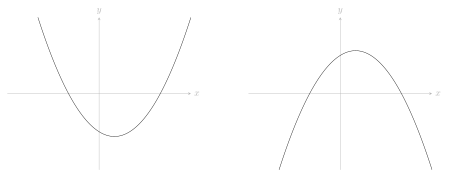
\includegraphics{./Figures/introtoquadratics-fig1.pdf}

}

\caption{\label{fig-1}A pair of parabolas. (left) A graph of a quadratic
\(ax^2 + bx + c\) where \(a > 0\). (right) A graph of a quadratic
\(ax^2 + bx + c\) where \(a < 0\).}

\end{figure}

It is very important to be able to identify the variable in a quadratic
equation, as well as the coefficients \(a,b,c\). In the course of your
mathematical study, it may be that the variable of a quadratic equation
is not only letters like \(x,y,z\), but squares or cubes like \(x^2\)
and \(y^3\), or even functions like \(e^x\), \(\cos(x)\), and
\(\sin(y)\).

\begin{tcolorbox}[enhanced jigsaw, bottomrule=.15mm, colback=white, opacityback=0, rightrule=.15mm, breakable, left=2mm, arc=.35mm, toprule=.15mm, colframe=quarto-callout-note-color-frame, leftrule=.75mm]
\begin{minipage}[t]{5.5mm}
\textcolor{quarto-callout-note-color}{\faInfo}
\end{minipage}%
\begin{minipage}[t]{\textwidth - 5.5mm}
You are given the quadratic equation \(2x^2 + 4x - 8 = 0\). The variable
of the quadratic equation is \(x\), and the coefficients are
\(a = 2, b = 4, c = -8\).\end{minipage}%
\end{tcolorbox}

\begin{tcolorbox}[enhanced jigsaw, bottomrule=.15mm, colback=white, opacityback=0, rightrule=.15mm, breakable, left=2mm, arc=.35mm, toprule=.15mm, colframe=quarto-callout-note-color-frame, leftrule=.75mm]
\begin{minipage}[t]{5.5mm}
\textcolor{quarto-callout-note-color}{\faInfo}
\end{minipage}%
\begin{minipage}[t]{\textwidth - 5.5mm}
Here, the equation \(y^4 - 10y^2 + 25 = 0\) may look like a quartic
equation, but it is actually a quadratic equation. Using the laws of
indices, you can rewrite the equation as \((y^2)^2 - 10y^2 + 25 = 0\).
Therefore, the variable of the quadratic equation is \(y^2\), and the
coefficients are \(a = 1\), \(b = -10\), \(c = 25\).\end{minipage}%
\end{tcolorbox}

\begin{tcolorbox}[enhanced jigsaw, bottomrule=.15mm, colback=white, opacityback=0, rightrule=.15mm, breakable, left=2mm, arc=.35mm, toprule=.15mm, colframe=quarto-callout-note-color-frame, leftrule=.75mm]
\begin{minipage}[t]{5.5mm}
\textcolor{quarto-callout-note-color}{\faInfo}
\end{minipage}%
\begin{minipage}[t]{\textwidth - 5.5mm}
You are given the equation \(-e^{2x} + 4e^{x} - 5 = 0\). Using the laws
of indices, you can rewrite the equation as
\(-(e^{x})^2 + 4e^x - 5 = 0\). The variable of the quadratic equation is
\(e^x\), and the coefficients are \(a = -1\), \(b = 4\), \(c = -5\).
This is not the only solution to the coefficients; you can multiply the
equation through by \(-1\) to get \((e^{x})^2 - 4e^x + 5 = 0\), which
gives \(a = 1\), \(b = -4\) and \(c = 5\). Both solutions are equally
valid.\end{minipage}%
\end{tcolorbox}

\begin{tcolorbox}[enhanced jigsaw, bottomrule=.15mm, colback=white, opacityback=0, rightrule=.15mm, breakable, left=2mm, arc=.35mm, toprule=.15mm, colframe=quarto-callout-note-color-frame, leftrule=.75mm]
\begin{minipage}[t]{5.5mm}
\textcolor{quarto-callout-note-color}{\faInfo}
\end{minipage}%
\begin{minipage}[t]{\textwidth - 5.5mm}
You are given the equation \(t+1 = \frac{4}{t-3}\). This really is a
quadratic equation! You can multiply both sides by \(x - 3\) to get
\[(t+1)(t+3) = 4\] You can then expand the brackets to get
\[t^2 + t + 3t + 3 = 4\] and so \(t^2 + 4t + 3 = 4\). Finally, you are
able to subtract \(4\) from both sides to get \(t^2 + 4t - 1 = 0\). It
follows that the variable of the quadratic equation is \(t\), and the
coefficients are \(a = 1\), \(b = 4\), \(c = -1\).\end{minipage}%
\end{tcolorbox}

\hypertarget{solving-a-quadratic-equation}{%
\subsection{Solving a quadratic
equation}\label{solving-a-quadratic-equation}}

To solve the quadratic equation, you could use one of three methods:

\begin{itemize}
\item
  You could \textbf{factorise} the quadratic equation
  \(ax^2 + bx + c = 0\) into linear equations \((mx + n)(px + q)\), then
  work out the roots when each of these linear equations is zero. See
  (Guide: Factorisation) for more.
\item
  You could \textbf{complete the square} in order to reduce the
  quadratic equation \(ax^2 + bx + c = 0\) into the form
  \((x + b/2a)^2 = d\), and then solve from there (not forgetting the
  negative root). See (Guide: Completing the square) for more.
\item
  You could \textbf{use the quadratic formula}; for a quadratic equation
  \(ax^2 + bx + c = 0\), the two roots to the quadratic equation are
  given by \[x = \frac{-b \pm \sqrt{b^2 - 4ac}}{2a}.\]
\end{itemize}

Each method is equally valid, but some may involve more work than
others. It is up to you to decide which method is best for each
quadratic you encounter; but it is thoroughly recommended that if you
are not sure which method is best, then the quadratic formula is the one
to choose. See \href{quadraticformula.qmd}{Guide: Using the quadratic
formula} for more.

\hypertarget{the-discriminant}{%
\subsection{The discriminant}\label{the-discriminant}}

What the roots of the quadratic formula look like are determined by the
term \(b^2 - 4ac\); this term has a special name.

\begin{tcolorbox}[enhanced jigsaw, bottomrule=.15mm, toprule=.15mm, coltitle=black, rightrule=.15mm, breakable, titlerule=0mm, arc=.35mm, toptitle=1mm, colback=white, opacitybacktitle=0.6, title=\textcolor{quarto-callout-note-color}{\faInfo}\hspace{0.5em}{The discriminant}, left=2mm, bottomtitle=1mm, opacityback=0, colbacktitle=quarto-callout-note-color!10!white, colframe=quarto-callout-note-color-frame, leftrule=.75mm]
The term \(D = b^2 - 4ac\) is known as the \textbf{discriminant} of the
quadratic equation \(ax^2 + bx + c = 0\).
\end{tcolorbox}

There are then three separate cases for solutions to quadratic
equations.

\begin{itemize}
\tightlist
\item
  If \(D = b^2 - 4ac\) is positive, then \(\sqrt{D}\) is a real number
  and the two roots of the quadratic equation \(ax^2 + bx + c = 0\) are
  \[x = \frac{-b + \sqrt{D}}{2a}\qquad\textsf{ and }\qquad x = \frac{-b - \sqrt{D}}{2a}\]
  These two roots are both real numbers and distinct from each other.
  You can observe this behaviour on a graph in Figure~\ref{fig-2}; the
  parabola crosses the \(x\)-axis in two places.
\end{itemize}

\begin{figure}

{\centering 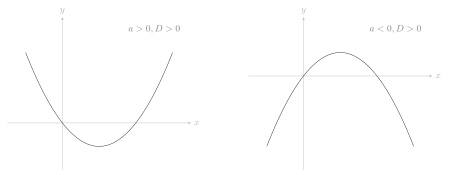
\includegraphics{./Figures/introtoquadratics-fig2.pdf}

}

\caption{\label{fig-2}A pair of parabolas. (left) A graph of a quadratic
\(ax^2 + bx + c\) where \(a > 0\) and \(D > 0\). (right) A graph of a
quadratic \(ax^2 + bx + c\) where \(a < 0\) and \(D > 0\).}

\end{figure}

\begin{itemize}
\tightlist
\item
  If \(D = b^2 - 4ac = 0\) is zero, then \(\sqrt{D} = 0\). In this case,
  the two roots of the quadratic equation \(ax^2 + bx + c = 0\) are
  \[x = \frac{-b}{2a} \qquad\textsf{ and }\qquad x = \frac{-b}{2a}\]
  These two roots are given by the same real number. To be sure that you
  express both roots, you can write `\(x = -b/2a\) twice'. You can
  observe this behaviour on a graph in Figure~\ref{fig-3}; the parabola
  touches the \(x\)-axis in exactly one place.
\end{itemize}

\begin{figure}

{\centering 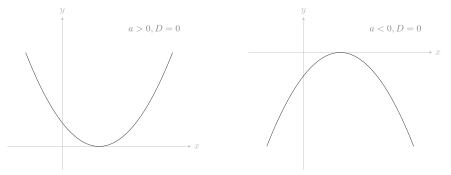
\includegraphics{./Figures/introtoquadratics-fig3.pdf}

}

\caption{\label{fig-3}A pair of parabolas. (left) A graph of a quadratic
\(ax^2 + bx + c\) where \(a > 0\) and \(D = 0\). (right) A graph of a
quadratic \(ax^2 + bx + c\) where \(a < 0\) and \(D = 0\).}

\end{figure}

\begin{itemize}
\tightlist
\item
  If \(D = b^2 - 4ac\) is negative, then \(\sqrt{D}\) is not a real
  number. In this case, the two roots of the quadratic equation are
  \textbf{complex numbers}. You can express the two roots of the
  quadratic equation by
  \[x = \frac{-b + i\sqrt{-D}}{2a}\qquad\textsf{ and }\qquad x = \frac{-b - i\sqrt{-D}}{2a}\]
  where \(i\) is the imaginary unit (so \(i^2 = -1\); see (Guide:
  Introduction to complex numbers)). In a graph, the parabola does not
  cross the \(x\)-axis at all; this indicates that there are no real
  solutions to this quadratic equation. See Figure~\ref{fig-4} for a
  picture.
\end{itemize}

\begin{figure}

{\centering 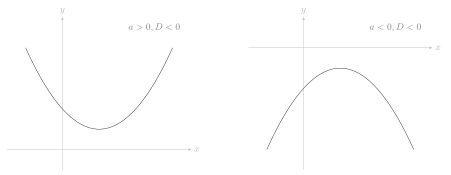
\includegraphics{./Figures/introtoquadratics-fig4.pdf}

}

\caption{\label{fig-4}A pair of parabolas. (left) A graph of a quadratic
\(ax^2 + bx + c\) where \(a > 0\) and \(D > 0\). (right) A graph of a
quadratic \(ax^2 + bx + c\) where \(a < 0\) and \(D < 0\).}

\end{figure}

\begin{tcolorbox}[enhanced jigsaw, bottomrule=.15mm, toprule=.15mm, coltitle=black, rightrule=.15mm, breakable, titlerule=0mm, arc=.35mm, toptitle=1mm, colback=white, opacitybacktitle=0.6, title=\textcolor{quarto-callout-warning-color}{\faExclamationTriangle}\hspace{0.5em}{Warning}, left=2mm, bottomtitle=1mm, opacityback=0, colbacktitle=quarto-callout-warning-color!10!white, colframe=quarto-callout-warning-color-frame, leftrule=.75mm]
You can use the discriminant to check how many roots a quadratic
equation has in the variable given to you. However, this is at most a
maximum number of solutions. Conditions on that variable may also reduce
the number of valid solutions, particularly if you have real valued
functions. For instance, since \(e^x > 0\) for all real number \(x\),
there are no solutions in \(x\) if you find \(e^x = -1\).
\end{tcolorbox}

Here's some examples of using the discriminant and known properties of
functions to rule out solutions.

\begin{tcolorbox}[enhanced jigsaw, bottomrule=.15mm, colback=white, opacityback=0, rightrule=.15mm, breakable, left=2mm, arc=.35mm, toprule=.15mm, colframe=quarto-callout-note-color-frame, leftrule=.75mm]
\begin{minipage}[t]{5.5mm}
\textcolor{quarto-callout-note-color}{\faInfo}
\end{minipage}%
\begin{minipage}[t]{\textwidth - 5.5mm}
In Example 1, you identified the coefficients of \(2x^2 + 4x - 8 = 0\)
as \(a = 2, b = 4, c = -8\). Using these, you can work out the value of
the discriminant \(D = b^2 - 4ac\) as
\[D = (4)^2 - 4(2)(-8) = 16 + 64 = 80.\] Since \(D = 80\), you can say
that this quadratic equation has two distinct real roots in \(x = r_1\)
and \(x = r_2\).\end{minipage}%
\end{tcolorbox}

\begin{tcolorbox}[enhanced jigsaw, bottomrule=.15mm, colback=white, opacityback=0, rightrule=.15mm, breakable, left=2mm, arc=.35mm, toprule=.15mm, colframe=quarto-callout-note-color-frame, leftrule=.75mm]
\begin{minipage}[t]{5.5mm}
\textcolor{quarto-callout-note-color}{\faInfo}
\end{minipage}%
\begin{minipage}[t]{\textwidth - 5.5mm}
In Example 2, you identified the coefficients of
\(y^4 - 10y^2 + 25 = 0\) as \(a = 1, b = -10, c = 25\), and the variable
as \(y^2\). Using these, you can work out the value of the discriminant
\(D = b^2 - 4ac\) as \[D = (-10)^2 - 4(1)(25) = 100 - 100 = 0.\] Since
\(D = 0\), you can say that this quadratic equation has at most one real
root \(r\) in terms of \(y^2\).

Whether or not the equation itself has real solutions in \(y\) depends
on whether \(r\) is positive or negative! You cannot take the square
root of a negative number, so if \(r\) is negative the equation has no
real solutions. If \(r\) is positive, then the equation has two real
roots in \(y\); that is, \(y = \pm\sqrt{r}\).\end{minipage}%
\end{tcolorbox}

\begin{tcolorbox}[enhanced jigsaw, bottomrule=.15mm, colback=white, opacityback=0, rightrule=.15mm, breakable, left=2mm, arc=.35mm, toprule=.15mm, colframe=quarto-callout-note-color-frame, leftrule=.75mm]
\begin{minipage}[t]{5.5mm}
\textcolor{quarto-callout-note-color}{\faInfo}
\end{minipage}%
\begin{minipage}[t]{\textwidth - 5.5mm}
In Example 3, you identified the coefficients of
\(-e^{2x} + 4e^{x} - 5 = 0\) as \(a = -1, b = 4, c = -5\), and the
variable as \(e^{x}\). Using these, you can work out the value of the
discriminant \(D = b^2 - 4ac\) as
\[D = (4)^2 - 4(-1)(-5) = 16 - 20 = -4.\] Since \(D = -4\), you can say
that this quadratic equation has complex roots.

This equation therefore has no real solutions in \(x\). This is because
\(e^x\) is real for any real \(x\); if \(e^x\) is complex, it follows
that \(x\) cannot be real.\end{minipage}%
\end{tcolorbox}

\begin{tcolorbox}[enhanced jigsaw, bottomrule=.15mm, colback=white, opacityback=0, rightrule=.15mm, breakable, left=2mm, arc=.35mm, toprule=.15mm, colframe=quarto-callout-note-color-frame, leftrule=.75mm]
\begin{minipage}[t]{5.5mm}
\textcolor{quarto-callout-note-color}{\faInfo}
\end{minipage}%
\begin{minipage}[t]{\textwidth - 5.5mm}
In Example 4, you rearranged the equation \(t+1 = \frac{4}{t-3}\) to
\(t^2 + 4t - 1 = 0\), and therefore identifed the coefficients as
\(a = 1, b = 4, c = -1\), and the variable as \(t\). Using these, you
can work out the value of the discriminant \(D = b^2 - 4ac\) as
\[D = (4)^2 - 4(1)(-1) = 16 + 4 = 20.\] Since \(D = 20\), you can say
that this quadratic equation has two distinct real roots in
\(t\).\end{minipage}%
\end{tcolorbox}

\hypertarget{quick-check-problems}{%
\subsection*{Quick check problems}\label{quick-check-problems}}
\addcontentsline{toc}{subsection}{Quick check problems}

\begin{enumerate}
\def\labelenumi{\arabic{enumi}.}
\item
  What is the discriminant of the quadratic equation
  \(x^2 - x - 1 = 0\)?
\item
  You are given the quadratic equation \(4h^2 - h + 101 = 0\). Identify
  the variable, and the coefficients \(a,b,c\).
\item
  You are given three statements below. Decide whether they are true or
  false.
\end{enumerate}

\begin{enumerate}
\def\labelenumi{(\alph{enumi})}
\item
  The quadratic equation \(m^2 + 4m + 4 = 0\) has two distinct real
  roots.
\item
  The quadratic equation \(m^2 - 4m - 4 = 0\) has exactly one real root.
\item
  The quadratic equation \(4m^2 + 4m + 4 = 0\) has no real roots.
\end{enumerate}

\href{qs-introtoquadratics.qmd}{For more questions on the subject,
please go to Questions: Introduction to quadratic equations.}

\hypertarget{further-reading}{%
\subsection*{Further reading}\label{further-reading}}
\addcontentsline{toc}{subsection}{Further reading}

\href{quadraticformula.html}{Guide: Using the quadratic formula}



\end{document}
